
\begin{figure}[ht]
\begin{center}
\begin{tabular}{cc}
\frame{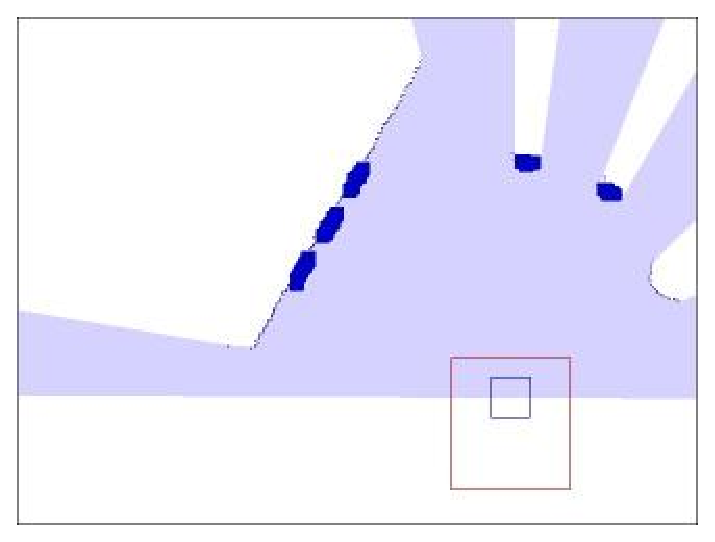
\epsfig{file=drivers/lasercspace-1.eps, height=40mm}} &
\frame{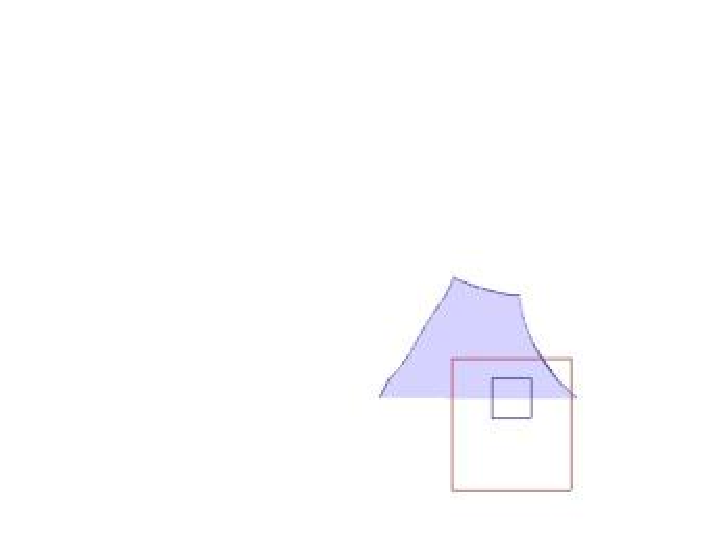
\epsfig{file=drivers/lasercspace-2.eps, height=40mm}} \\
(a) & (b) \\
\end{tabular}
\caption{(a) Standard laser scan.  (b) The corresponding C-space scan 
for a robot of radius 0.05~m}
\label{fig:lasercspace}
\end{center}
\end{figure}

\subsection*{Synopsis}

The lasercspace driver processes a laser scan to compute the
configuration space (`C-space') boundary.  That is, it shortens the
range of each laser scan such that the resultant scan delimits the
obstacle-free portion of the robot's configuration space.  This driver
is particular useful for writing obstacle avoidance algorithms, since the
robot may safely move to any point in the obstacle-free portion of the 
configuration space.

Note that driver computes the configuration space for a robot of some
fixed radius; this radius may be set in the configuration file.


\subsection*{Interfaces}

\noindent Supported interfaces:
\begin{itemize}
\item {\tt laser}
\end{itemize}

\noindent Required devices:
\begin{itemize}
\item {\tt laser}
\end{itemize}

\noindent Supported configuration requests:
\begin{itemize}
\item \verb+PLAYER_LASER_GET_GEOM+
\end{itemize}

\subsection*{Configuration file options}

\begin{center}
{\small \begin{tabularx}{\columnwidth}{|l|l|c|X|}
\hline
Name & Type & Default & Meaning\\
\hline
\verb+laser+ & integer & 0 & Index of the laser device to use. \\
\verb+radius+ & length & 0.50 & Robot radius. \\
\hline
\end{tabularx}}
\end{center}


\subsection*{Notes}
